%%
%% Automatically generated file from DocOnce source
%% (https://github.com/doconce/doconce/)
%% doconce format latex week1.do.txt --latex_title_layout=beamer --latex_table_format=footnotesize --no_mako
%%
% #ifdef PTEX2TEX_EXPLANATION
%%
%% The file follows the ptex2tex extended LaTeX format, see
%% ptex2tex: https://code.google.com/p/ptex2tex/
%%
%% Run
%%      ptex2tex myfile
%% or
%%      doconce ptex2tex myfile
%%
%% to turn myfile.p.tex into an ordinary LaTeX file myfile.tex.
%% (The ptex2tex program: https://code.google.com/p/ptex2tex)
%% Many preprocess options can be added to ptex2tex or doconce ptex2tex
%%
%%      ptex2tex -DMINTED myfile
%%      doconce ptex2tex myfile envir=minted
%%
%% ptex2tex will typeset code environments according to a global or local
%% .ptex2tex.cfg configure file. doconce ptex2tex will typeset code
%% according to options on the command line (just type doconce ptex2tex to
%% see examples). If doconce ptex2tex has envir=minted, it enables the
%% minted style without needing -DMINTED.
% #endif

% #define PREAMBLE

% #ifdef PREAMBLE
%-------------------- begin preamble ----------------------

\documentclass[%
oneside,                 % oneside: electronic viewing, twoside: printing
final,                   % draft: marks overfull hboxes, figures with paths
10pt]{article}

\listfiles               %  print all files needed to compile this document

\usepackage{relsize,makeidx,color,setspace,amsmath,amsfonts,amssymb}
\usepackage[table]{xcolor}
\usepackage{bm,ltablex,microtype}

\usepackage[pdftex]{graphicx}

\usepackage[T1]{fontenc}
%\usepackage[latin1]{inputenc}
\usepackage{ucs}
\usepackage[utf8x]{inputenc}

\usepackage{lmodern}         % Latin Modern fonts derived from Computer Modern

% Hyperlinks in PDF:
\definecolor{linkcolor}{rgb}{0,0,0.4}
\usepackage{hyperref}
\hypersetup{
    breaklinks=true,
    colorlinks=true,
    linkcolor=linkcolor,
    urlcolor=linkcolor,
    citecolor=black,
    filecolor=black,
    %filecolor=blue,
    pdfmenubar=true,
    pdftoolbar=true,
    bookmarksdepth=3   % Uncomment (and tweak) for PDF bookmarks with more levels than the TOC
    }
%\hyperbaseurl{}   % hyperlinks are relative to this root

\setcounter{tocdepth}{2}  % levels in table of contents

% Tricks for having figures close to where they are defined:
% 1. define less restrictive rules for where to put figures
\setcounter{topnumber}{2}
\setcounter{bottomnumber}{2}
\setcounter{totalnumber}{4}
\renewcommand{\topfraction}{0.95}
\renewcommand{\bottomfraction}{0.95}
\renewcommand{\textfraction}{0}
\renewcommand{\floatpagefraction}{0.75}
% floatpagefraction must always be less than topfraction!
% 2. ensure all figures are flushed before next section
\usepackage[section]{placeins}
% 3. enable begin{figure}[H] (often leads to ugly pagebreaks)
%\usepackage{float}\restylefloat{figure}

% --- fancyhdr package for fancy headers ---
\usepackage{fancyhdr}
\fancyhf{} % sets both header and footer to nothing
\renewcommand{\headrulewidth}{0pt}
\fancyfoot[LE,RO]{\thepage}
% Ensure copyright on titlepage (article style) and chapter pages (book style)
\fancypagestyle{plain}{
  \fancyhf{}
  \fancyfoot[C]{{\footnotesize \copyright\ 1999-2024, Morten Hjorth-Jensen. Released under CC Attribution-NonCommercial 4.0 license}}
%  \renewcommand{\footrulewidth}{0mm}
  \renewcommand{\headrulewidth}{0mm}
}
% Ensure copyright on titlepages with \thispagestyle{empty}
\fancypagestyle{empty}{
  \fancyhf{}
  \fancyfoot[C]{{\footnotesize \copyright\ 1999-2024, Morten Hjorth-Jensen. Released under CC Attribution-NonCommercial 4.0 license}}
  \renewcommand{\footrulewidth}{0mm}
  \renewcommand{\headrulewidth}{0mm}
}

\pagestyle{fancy}


\usepackage[framemethod=TikZ]{mdframed}

% --- begin definitions of admonition environments ---

% Admonition style "mdfbox" is an oval colored box based on mdframed
% "notice" admon
\colorlet{mdfbox_notice_background}{gray!5}
\newmdenv[
  skipabove=15pt,
  skipbelow=15pt,
  outerlinewidth=0,
  backgroundcolor=mdfbox_notice_background,
  linecolor=black,
  linewidth=2pt,       % frame thickness
  frametitlebackgroundcolor=mdfbox_notice_background,
  frametitlerule=true,
  frametitlefont=\normalfont\bfseries,
  shadow=false,        % frame shadow?
  shadowsize=11pt,
  leftmargin=0,
  rightmargin=0,
  roundcorner=5,
  needspace=0pt,
]{notice_mdfboxmdframed}

\newenvironment{notice_mdfboxadmon}[1][]{
\begin{notice_mdfboxmdframed}[frametitle=#1]
}
{
\end{notice_mdfboxmdframed}
}

% Admonition style "mdfbox" is an oval colored box based on mdframed
% "summary" admon
\colorlet{mdfbox_summary_background}{gray!5}
\newmdenv[
  skipabove=15pt,
  skipbelow=15pt,
  outerlinewidth=0,
  backgroundcolor=mdfbox_summary_background,
  linecolor=black,
  linewidth=2pt,       % frame thickness
  frametitlebackgroundcolor=mdfbox_summary_background,
  frametitlerule=true,
  frametitlefont=\normalfont\bfseries,
  shadow=false,        % frame shadow?
  shadowsize=11pt,
  leftmargin=0,
  rightmargin=0,
  roundcorner=5,
  needspace=0pt,
]{summary_mdfboxmdframed}

\newenvironment{summary_mdfboxadmon}[1][]{
\begin{summary_mdfboxmdframed}[frametitle=#1]
}
{
\end{summary_mdfboxmdframed}
}

% Admonition style "mdfbox" is an oval colored box based on mdframed
% "warning" admon
\colorlet{mdfbox_warning_background}{gray!5}
\newmdenv[
  skipabove=15pt,
  skipbelow=15pt,
  outerlinewidth=0,
  backgroundcolor=mdfbox_warning_background,
  linecolor=black,
  linewidth=2pt,       % frame thickness
  frametitlebackgroundcolor=mdfbox_warning_background,
  frametitlerule=true,
  frametitlefont=\normalfont\bfseries,
  shadow=false,        % frame shadow?
  shadowsize=11pt,
  leftmargin=0,
  rightmargin=0,
  roundcorner=5,
  needspace=0pt,
]{warning_mdfboxmdframed}

\newenvironment{warning_mdfboxadmon}[1][]{
\begin{warning_mdfboxmdframed}[frametitle=#1]
}
{
\end{warning_mdfboxmdframed}
}

% Admonition style "mdfbox" is an oval colored box based on mdframed
% "question" admon
\colorlet{mdfbox_question_background}{gray!5}
\newmdenv[
  skipabove=15pt,
  skipbelow=15pt,
  outerlinewidth=0,
  backgroundcolor=mdfbox_question_background,
  linecolor=black,
  linewidth=2pt,       % frame thickness
  frametitlebackgroundcolor=mdfbox_question_background,
  frametitlerule=true,
  frametitlefont=\normalfont\bfseries,
  shadow=false,        % frame shadow?
  shadowsize=11pt,
  leftmargin=0,
  rightmargin=0,
  roundcorner=5,
  needspace=0pt,
]{question_mdfboxmdframed}

\newenvironment{question_mdfboxadmon}[1][]{
\begin{question_mdfboxmdframed}[frametitle=#1]
}
{
\end{question_mdfboxmdframed}
}

% Admonition style "mdfbox" is an oval colored box based on mdframed
% "block" admon
\colorlet{mdfbox_block_background}{gray!5}
\newmdenv[
  skipabove=15pt,
  skipbelow=15pt,
  outerlinewidth=0,
  backgroundcolor=mdfbox_block_background,
  linecolor=black,
  linewidth=2pt,       % frame thickness
  frametitlebackgroundcolor=mdfbox_block_background,
  frametitlerule=true,
  frametitlefont=\normalfont\bfseries,
  shadow=false,        % frame shadow?
  shadowsize=11pt,
  leftmargin=0,
  rightmargin=0,
  roundcorner=5,
  needspace=0pt,
]{block_mdfboxmdframed}

\newenvironment{block_mdfboxadmon}[1][]{
\begin{block_mdfboxmdframed}[frametitle=#1]
}
{
\end{block_mdfboxmdframed}
}

% --- end of definitions of admonition environments ---

% prevent orhpans and widows
\clubpenalty = 10000
\widowpenalty = 10000

% --- end of standard preamble for documents ---


% insert custom LaTeX commands...

\raggedbottom
\makeindex

%-------------------- end preamble ----------------------

\begin{document}

% matching end for #ifdef PREAMBLE
% #endif

\newcommand{\exercisesection}[1]{\subsection*{#1}}


% ------------------- main content ----------------------



% ----------------- title -------------------------

\title{January 15-19: Advanced machine learning and data analysis for the physical sciences}

% ----------------- author(s) -------------------------

\author{Morten Hjorth-Jensen\inst{1,2}}
\institute{Department of Physics and Center for Computing in Science Education, University of Oslo, Norway\inst{1}
\and
Department of Physics and Astronomy and Facility for Rare Isotope Beams, Michigan State University, East Lansing, Michigan, USA\inst{2}}
% ----------------- end author(s) -------------------------

\date{FYS5429/9429, Spring 2024
% <optional titlepage figure>
% <optional copyright>
}

% !split
\subsection{Overview of first week, January 15-19, 2024}

\begin{block}{}
\begin{enumerate}
 \item Presentation of course

 \item Discussion of possible projects and presentation of participants

 \item Deep learning methods, mathematics and  review of neural networks
\end{enumerate}

\noindent
\end{block}

% !split
\subsection{Practicalities}

\begin{enumerate}
\item Lectures Tuesday 1015am-12pm, room FØ434, Department of Physics

\item We plan to work on two projects which will define the content of the course, the format can be agreed upon by the participants

\item No exam, only two projects. Each projects counts 1/2 of the final grade.

\item All info at the GitHub address \href{{https://github.com/CompPhysics/AdvancedMachineLearning}}{\nolinkurl{https://github.com/CompPhysics/AdvancedMachineLearning}}
\end{enumerate}

\noindent
% !split
\subsection{Deep learning methods covered, tentative}

\begin{enumerate}
\item \textbf{Deep learning, classics}
\begin{enumerate}

 \item Feed forward neural networks and its mathematics (NNs)

 \item Convolutional neural networks (CNNs)

 \item Recurrent neural networks (RNNs)

 \item Autoencoders and principal component analysis

\end{enumerate}

\noindent
\item \textbf{Deep learning, generative methods}
\begin{enumerate}

 \item Basics of generative models

 \item Boltzmann machines and energy based methods

 \item Diffusion models (tentative)

 \item Variational autoencoders (VAEe)

 \item Generative Adversarial Networks (GANs)

 \item Autoregressive methods (tentative)

\end{enumerate}

\noindent
\item \textbf{Physical Sciences (often just called Physics informed) informed machine learning}
\end{enumerate}

\noindent
% !split
\subsection{\href{{https://jenfb.github.io/bkmr/overview.html}}{Additional topics:  Kernel regression (Gaussian processes) and Bayesian statistics}}

Kernel machine regression (KMR), also called Gaussian process
regression, is a popular tool in the machine learning literature. The
main idea behind KMR is to flexibly model the relationship between a
large number of variables and a particular outcome (dependent
variable).

% !split
\subsection{Scientific Machine Learning}

An important and emerging field is what has been dubbed as scientific ML, see the article by Deiana et al \href{{https://doi.org/10.3389/fdata.2022.787421}}{Applications and Techniques for Fast Machine Learning in Science, Big Data 5, 787421 (2022)}

\begin{block}{}
The authors discuss applications and techniques for fast machine
learning (ML) in science -- the concept of integrating power ML
methods into the real-time experimental data processing loop to
accelerate scientific discovery. The report covers three main areas

\begin{enumerate}
\item applications for fast ML across a number of scientific domains;

\item techniques for training and implementing performant and resource-efficient ML algorithms;

\item and computing architectures, platforms, and technologies for deploying these algorithms.
\end{enumerate}

\noindent
\end{block}

% !split
\subsection{Physics driven Machine Learning}

Another hot topic is what has loosely been dubbed \textbf{Physics-driven deep learning}. See the recent work on \href{{https://www.nature.com/articles/s42256-021-00302-5}}{Learning nonlinear operators via DeepONet based on the universal approximation theorem of operators, Nature Machine Learning, vol 3, 218 (2021)}.

\begin{block}{From their abstract }
A less known but powerful result is that an NN with a single hidden layer can accurately approximate any nonlinear continuous operator. This universal approximation theorem of operators is suggestive of the structure and potential of deep neural networks (DNNs) in learning continuous operators or complex systems from streams of scattered data. ...  We demonstrate that DeepONet can learn various explicit operators, such as integrals and fractional Laplacians, as well as implicit operators that represent deterministic and stochastic differential equations. 
\end{block}

% !split
\subsection{Good books with hands-on material and codes}
\begin{block}{}
\begin{itemize}
\item \href{{https://sebastianraschka.com/blog/2022/ml-pytorch-book.html}}{Sebastian Rashcka et al, Machine learning with Sickit-Learn and PyTorch}

\item \href{{https://www.oreilly.com/library/view/generative-deep-learning/9781098134174/ch01.html}}{David Foster, Generative Deep Learning with TensorFlow}

\item \href{{https://github.com/PacktPublishing/Hands-On-Generative-AI-with-Python-and-TensorFlow-2}}{Bali and Gavras, Generative AI with Python and TensorFlow 2}
\end{itemize}

\noindent
\end{block}

All three books have GitHub addresses from where  one can download all codes. We will borrow most of the material from these three texts as well as 
from Goodfellow, Bengio and Courville's text \href{{https://www.deeplearningbook.org/}}{Deep Learning}

% !split
\subsection{Machine learning. A simple perspective on the interface between ML and Physics, HPC is essential}

\vspace{6mm}

% inline figure
\centerline{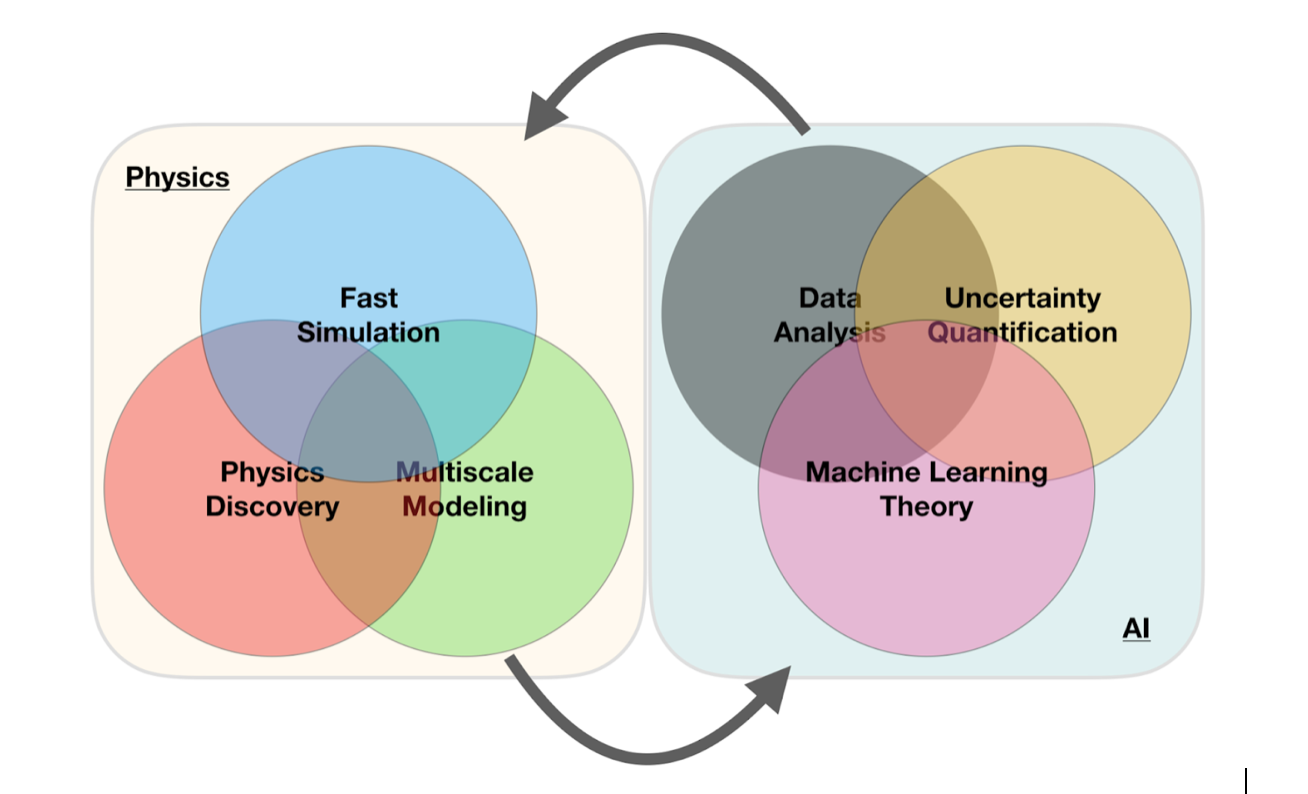
\includegraphics[width=1.0\linewidth]{figures/mlimage.png}}

\vspace{6mm}

% !split
\subsection{AI/ML and some statements you may have heard (and what do they mean?)}

\begin{enumerate}
\item Fei-Fei Li on ImageNet: \textbf{map out the entire world of objects} (\href{{https://cacm.acm.org/news/219702-the-data-that-transformed-ai-research-and-possibly-the-world/fulltext}}{The data that transformed AI research})

\item Russell and Norvig in their popular textbook: \textbf{relevant to any intellectual task; it is truly a universal field} (\href{{http://aima.cs.berkeley.edu/}}{Artificial Intelligence, A modern approach})

\item Woody Bledsoe puts it more bluntly: \textbf{in the long run, AI is the only science} (quoted in Pamilla McCorduck, \href{{https://www.pamelamccorduck.com/machines-who-think}}{Machines who think})
\end{enumerate}

\noindent
If you wish to have a critical read on AI/ML from a societal point of view, see \href{{https://www.katecrawford.net/}}{Kate Crawford's recent text Atlas of AI}. See also \href{{https://www.nationaldefensemagazine.org/articles/2023/3/24/ukraine-a-living-lab-for-ai-warfare}}{\nolinkurl{https://www.nationaldefensemagazine.org/articles/2023/3/24/ukraine-a-living-lab-for-ai-warfare}}

\textbf{Here: with AI/ML we intend a collection of machine learning methods with an emphasis on statistical learning and data analysis}

% !split
\subsection{Types of machine learning}

\begin{block}{}
The approaches to machine learning are many, but are often split into two main categories. 
In \emph{supervised learning} we know the answer to a problem,
and let the computer deduce the logic behind it. On the other hand, \emph{unsupervised learning}
is a method for finding patterns and relationship in data sets without any prior knowledge of the system.

An emerging  third category is  \emph{reinforcement learning}. This is a paradigm 
of learning inspired by behavioural psychology, where learning is achieved by trial-and-error, 
solely from rewards and punishment.
\end{block}

% !split
\subsection{Main categories}
\begin{block}{}
Another way to categorize machine learning tasks is to consider the desired output of a system.
Some of the most common tasks are:

\begin{itemize}
  \item Classification: Outputs are divided into two or more classes. The goal is to   produce a model that assigns inputs into one of these classes. An example is to identify  digits based on pictures of hand-written ones. Classification is typically supervised learning.

  \item Regression: Finding a functional relationship between an input data set and a reference data set.   The goal is to construct a function that maps input data to continuous output values.

  \item Clustering: Data are divided into groups with certain common traits, without knowing the different groups beforehand.  It is thus a form of unsupervised learning.
\end{itemize}

\noindent
\end{block}

% !split
\subsection{The plethora  of machine learning algorithms/methods}

\begin{enumerate}
\item Deep learning: Neural Networks (NNs), Convolutional NNs, Recurrent NNs, Transformers, Boltzmann machines, autoencoders and variational autoencoders  and generative adversarial networks and other generative models 

\item Bayesian statistics and Bayesian Machine Learning, Bayesian experimental design, Bayesian Regression models, Bayesian neural networks, Gaussian processes and much more

\item Dimensionality reduction (Principal component analysis), Clustering Methods and more

\item Ensemble Methods, Random forests, bagging and voting methods, gradient boosting approaches 

\item Linear and logistic regression, Kernel methods, support vector machines and more

\item Reinforcement Learning; Transfer Learning and more 
\end{enumerate}

\noindent
% !split
\subsection{What Is Generative Modeling?}

Generative modeling can be broadly defined as follows:

Generative modeling is a branch of machine learning that involves
training a model to produce new data that is similar to a given
dataset.

What does this mean in practice? Suppose we have a dataset containing
photos of horses. We can train a generative model on this dataset to
capture the rules that govern the complex relationships between pixels
in images of horses. Then we can sample from this model to create
novel, realistic images of horses that did not exist in the original
dataset. 

% !split
\subsection{Example of generative modeling, \href{{https://www.oreilly.com/library/view/generative-deep-learning/9781098134174/ch01.html}}{taken from Generative Deeep Learning by David Foster}}

\vspace{6mm}

% inline figure
\centerline{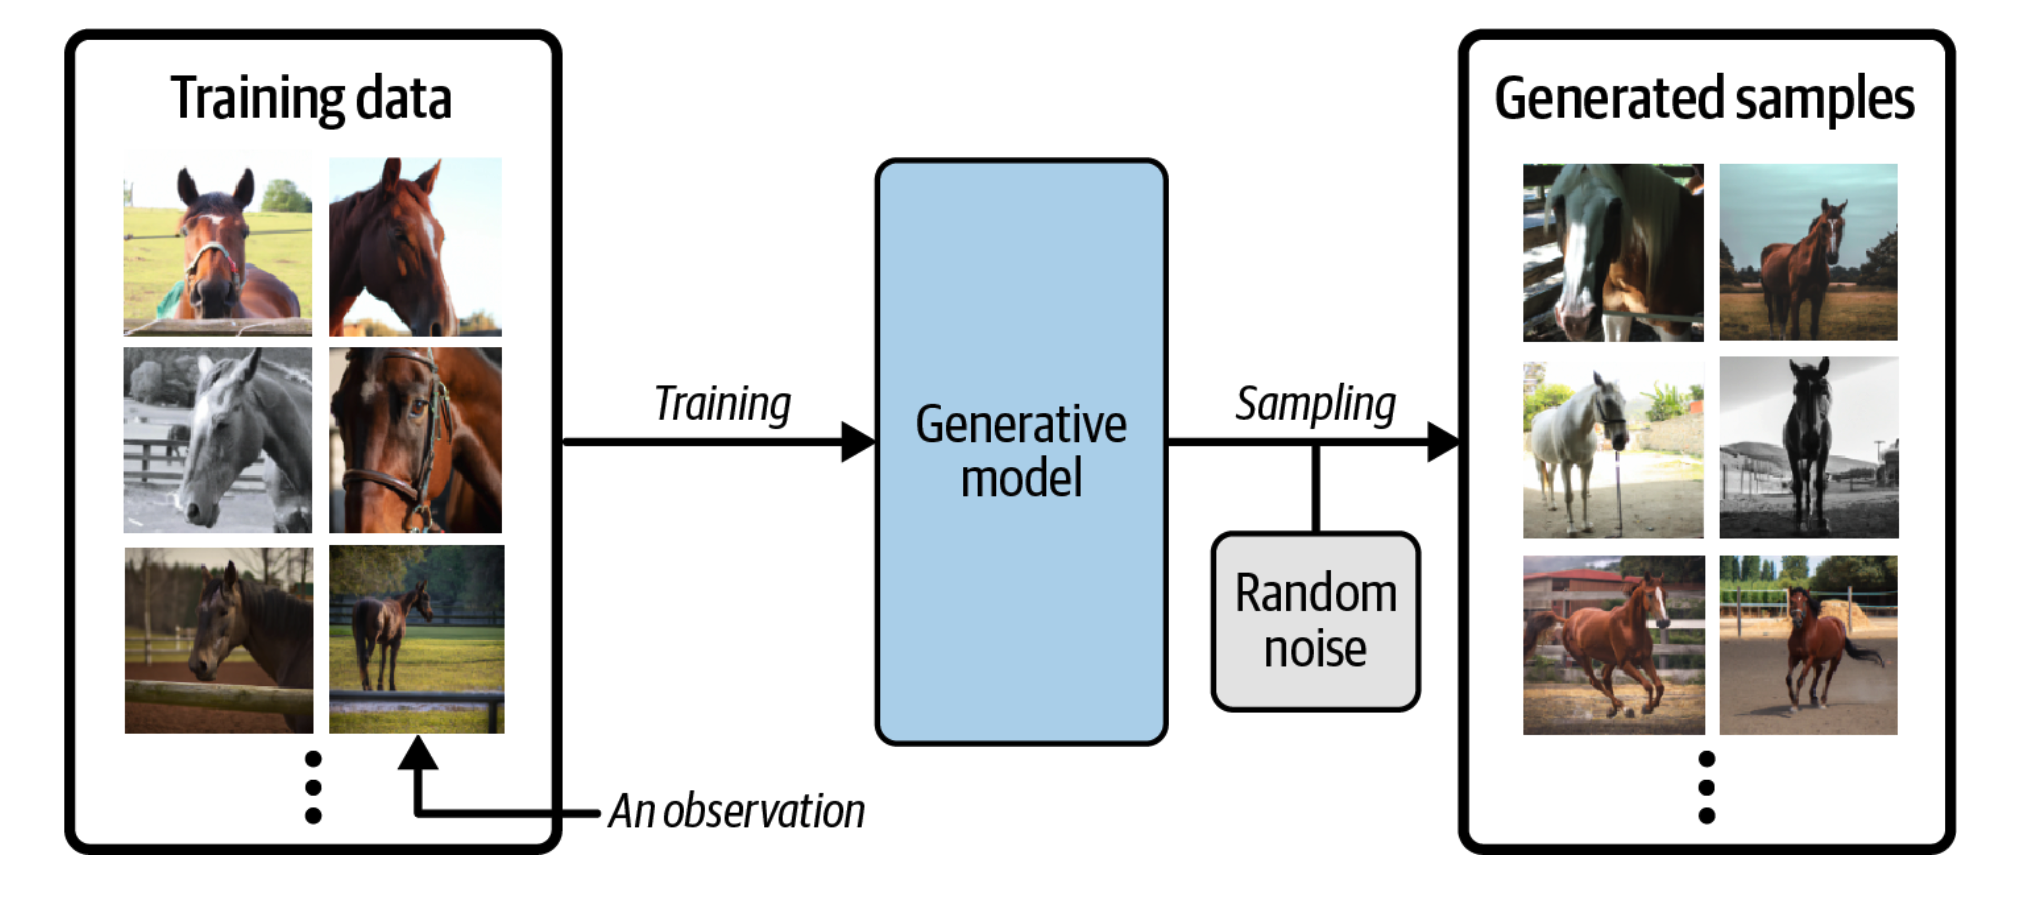
\includegraphics[width=1.0\linewidth]{figures/generativelearning.png}}

\vspace{6mm}

% !split
\subsection{Generative Modeling}

In order to build a generative model, we require a dataset consisting
of many examples of the entity we are trying to generate. This is
known as the training data, and one such data point is called an
observation.

Each observation consists of many features. For an image generation
problem, the features are usually the individual pixel values; for a
text generation problem, the features could be individual words or
groups of letters. It is our goal to build a model that can generate
new sets of features that look as if they have been created using the
same rules as the original data. Conceptually, for image generation
this is an incredibly difficult task, considering the vast number of
ways that individual pixel values can be assigned and the relatively
tiny number of such arrangements that constitute an image of the
entity we are trying to generate.

% !split
\subsection{Generative Versus Discriminative Modeling}

In order to truly understand what generative modeling aims to achieve
and why this is important, it is useful to compare it to its
counterpart, discriminative modeling. If you have studied machine
learning, most problems you will have faced will have most likely been
discriminative in nature. 

% !split
\subsection{Example of discriminative modeling, \href{{https://www.oreilly.com/library/view/generative-deep-learning/9781098134174/ch01.html}}{taken from Generative Deeep Learning by David Foster}}

\vspace{6mm}

% inline figure
\centerline{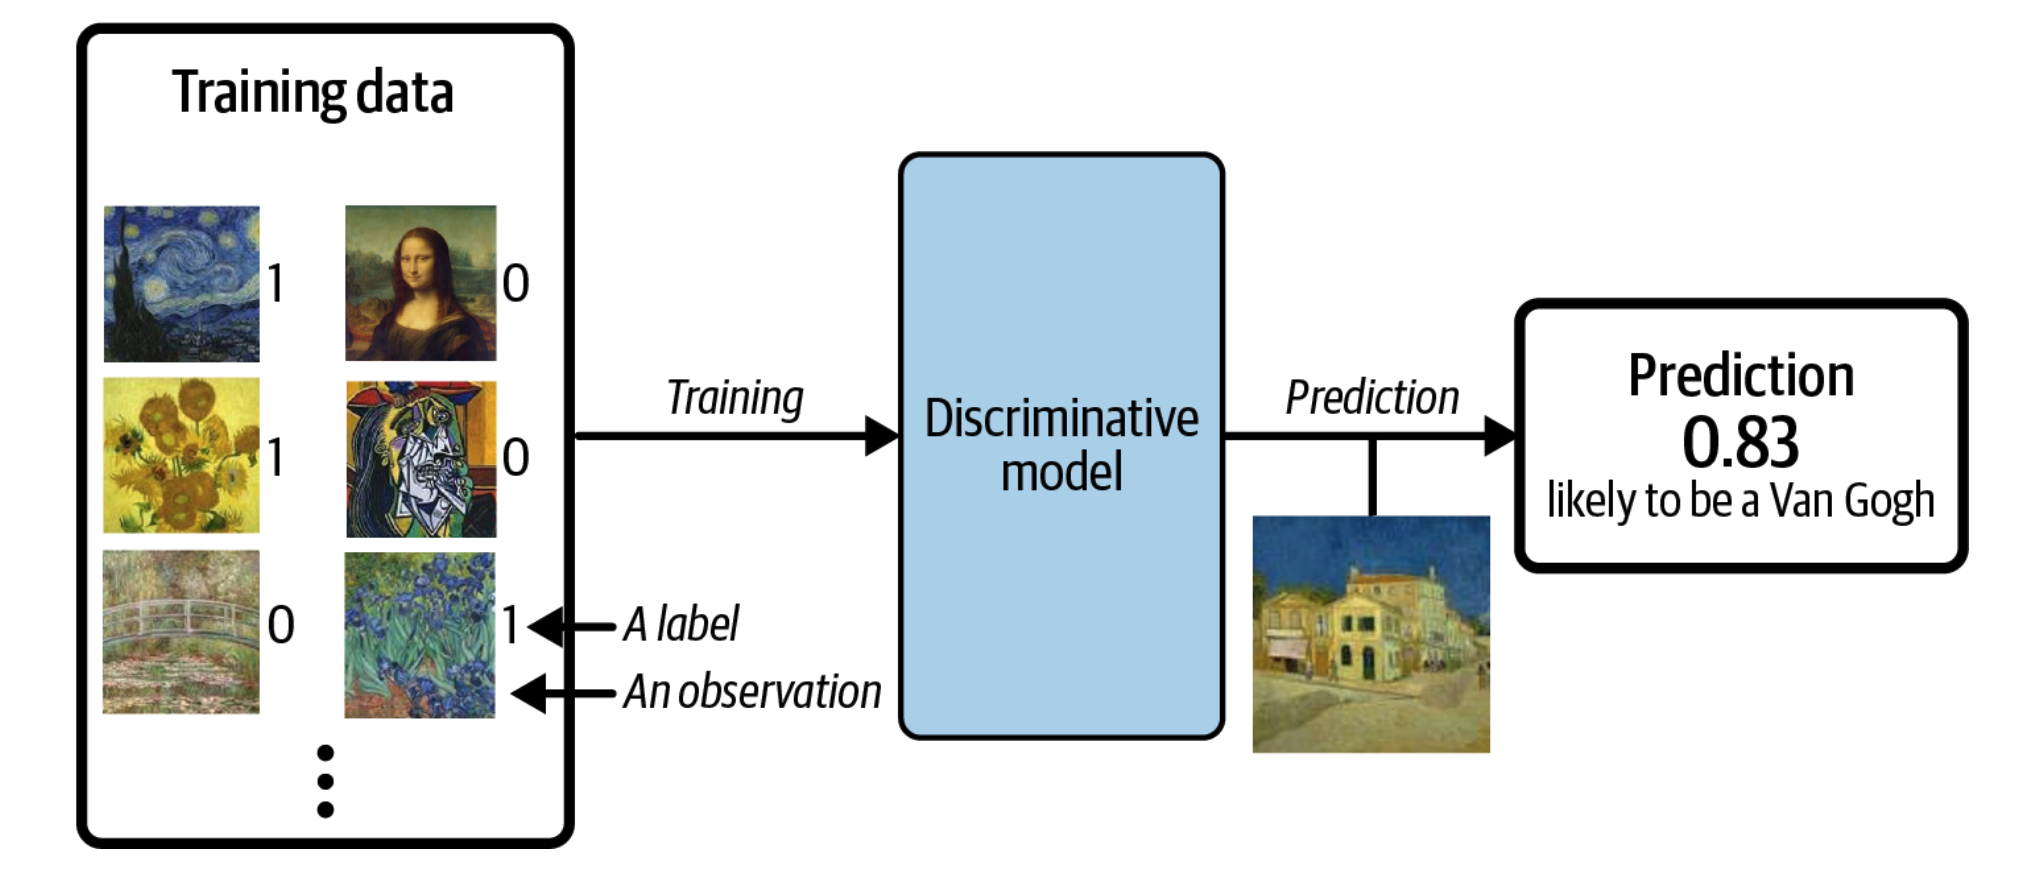
\includegraphics[width=1.0\linewidth]{figures/standarddeeplearning.png}}

\vspace{6mm}

% !split
\subsection{Discriminative Modeling}

When performing discriminative modeling, each observation in the
training data has a label. For a binary classification problem such as
our data could be labeled as ones and zeros. Our model then learns how to
discriminate between these two groups and outputs the probability that
a new observation has label 1 or 0

In contrast, generative modeling doesn’t require the dataset to be
labeled because it concerns itself with generating entirely new
data (for example an image), rather than trying to predict a label for say  a given image.

% !split
\subsection{Taxonomy of generative deep learning, \href{{https://www.oreilly.com/library/view/generative-deep-learning/9781098134174/ch01.html}}{taken from Generative Deep Learning by David Foster}}

\vspace{6mm}

% inline figure
\centerline{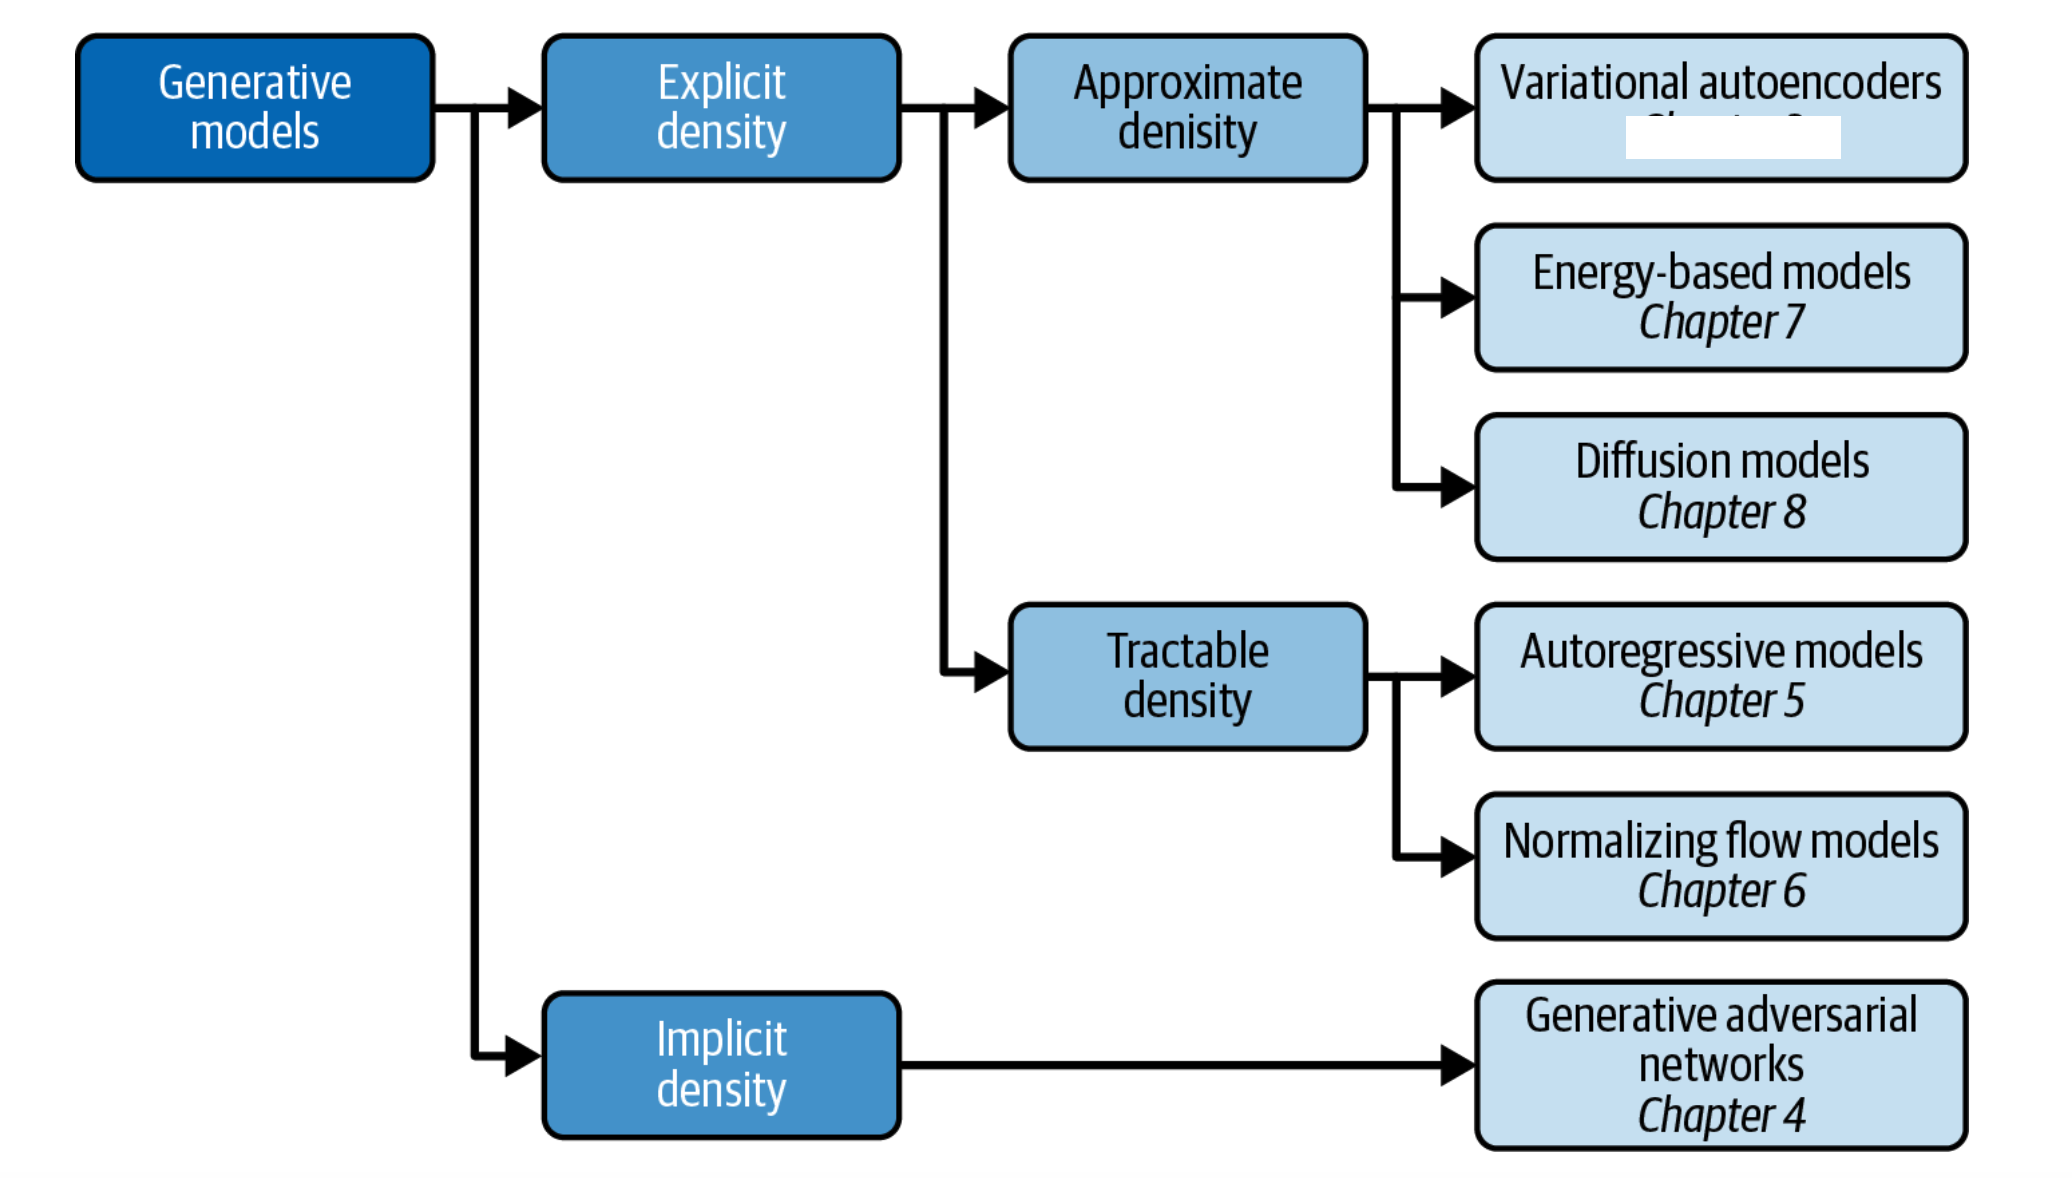
\includegraphics[width=1.0\linewidth]{figures/generativemodels.png}}

\vspace{6mm}

% !split
\subsection{What are the basic ingredients?}
\begin{block}{}
Almost every problem in ML and data science starts with the same ingredients:
\begin{itemize}
\item The dataset $\mathbf{x}$ (could be some observable quantity of the system we are studying)

\item A model which is a function of a set of parameters $\mathbf{\alpha}$ that relates to the dataset, say a likelihood  function $p(\mathbf{x}\vert \mathbf{\alpha})$ or just a simple model $f(\mathbf{\alpha})$

\item A so-called \textbf{loss/cost/risk} function $\mathcal{C} (\mathbf{x}, f(\mathbf{\alpha}))$ which allows us to decide how well our model represents the dataset. 
\end{itemize}

\noindent
We seek to minimize the function $\mathcal{C} (\mathbf{x}, f(\mathbf{\alpha}))$ by finding the parameter values which minimize $\mathcal{C}$. This leads to  various minimization algorithms. It may surprise many, but at the heart of all machine learning algortihms there is an optimization problem. 
\end{block}

% !split
\subsection{Low-level machine learning, the family of ordinary least squares methods}

Our data which we want to apply a machine learning method on, consist
of a set of inputs $\bm{x}^T=[x_0,x_1,x_2,\dots,x_{n-1}]$ and the
outputs we want to model $\bm{y}^T=[y_0,y_1,y_2,\dots,y_{n-1}]$.
We assume  that the output data can be represented (for a regression case) by a continuous function $f$
through
\[
\bm{y}=f(\bm{x})+\bm{\epsilon}.
\]

% !split
\subsection{Setting up the equations}

In linear regression we approximate the unknown function with another
continuous function $\tilde{\bm{y}}(\bm{x})$ which depends linearly on
some unknown parameters
$\bm{\theta}^T=[\theta_0,\theta_1,\theta_2,\dots,\theta_{p-1}]$.

The input data can be organized in terms of a so-called design matrix 
with an approximating function $\bm{\tilde{y}}$ 
\[
\bm{\tilde{y}}= \bm{X}\bm{\theta},
\]

% !split
\subsection{The objective/cost/loss function}

The  simplest approach is the mean squared error
\[
C(\bm{\Theta})=\frac{1}{n}\sum_{i=0}^{n-1}\left(y_i-\tilde{y}_i\right)^2=\frac{1}{n}\left\{\left(\bm{y}-\bm{\tilde{y}}\right)^T\left(\bm{y}-\bm{\tilde{y}}\right)\right\},
\]
or using the matrix $\bm{X}$ and in a more compact matrix-vector notation as
\[
C(\bm{\Theta})=\frac{1}{n}\left\{\left(\bm{y}-\bm{X}\bm{\theta}\right)^T\left(\bm{y}-\bm{X}\bm{\theta}\right)\right\}.
\]
This function represents one of many possible ways to define the so-called cost function.

% !split
\subsection{Training solution}

Optimizing with respect to the unknown paramters $\theta_j$ we get 
\[
\bm{X}^T\bm{y} = \bm{X}^T\bm{X}\bm{\theta},  
\]
and if the matrix $\bm{X}^T\bm{X}$ is invertible we have the optimal values
\[
\hat{\bm{\theta}} =\left(\bm{X}^T\bm{X}\right)^{-1}\bm{X}^T\bm{y}.
\]

We say we 'learn' the unknown paramters $\bm{\theta}$ from the last equation.

% !split
\subsection{Ridge and LASSO Regression}

Our optimization problem is
\[
{\displaystyle \min_{\bm{\theta}\in {\mathbb{R}}^{p}}}\frac{1}{n}\left\{\left(\bm{y}-\bm{X}\bm{\theta}\right)^T\left(\bm{y}-\bm{X}\bm{\theta}\right)\right\}.
\]
or we can state it as
\[
{\displaystyle \min_{\bm{\theta}\in
{\mathbb{R}}^{p}}}\frac{1}{n}\sum_{i=0}^{n-1}\left(y_i-\tilde{y}_i\right)^2=\frac{1}{n}\vert\vert \bm{y}-\bm{X}\bm{\theta}\vert\vert_2^2,
\]
where we have used the definition of  a norm-2 vector, that is
\[
\vert\vert \bm{x}\vert\vert_2 = \sqrt{\sum_i x_i^2}. 
\]

% !split
\subsection{From OLS to Ridge and Lasso}

By minimizing the above equation with respect to the parameters
$\bm{\theta}$ we could then obtain an analytical expression for the
parameters $\bm{\theta}$.  We can add a regularization parameter $\lambda$ by
defining a new cost function to be optimized, that is

\[
{\displaystyle \min_{\bm{\theta}\in
{\mathbb{R}}^{p}}}\frac{1}{n}\vert\vert \bm{y}-\bm{X}\bm{\theta}\vert\vert_2^2+\lambda\vert\vert \bm{\theta}\vert\vert_2^2
\]

which leads to the Ridge regression minimization problem where we
require that $\vert\vert \bm{\theta}\vert\vert_2^2\le t$, where $t$ is
a finite number larger than zero. We do not include such a constraints in the discussions here.

% !split
\subsection{Lasso regression}

Defining

\[
C(\bm{X},\bm{\theta})=\frac{1}{n}\vert\vert \bm{y}-\bm{X}\bm{\theta}\vert\vert_2^2+\lambda\vert\vert \bm{\theta}\vert\vert_1,
\]
we have a new optimization equation
\[
{\displaystyle \min_{\bm{\theta}\in
{\mathbb{R}}^{p}}}\frac{1}{n}\vert\vert \bm{y}-\bm{X}\bm{\theta}\vert\vert_2^2+\lambda\vert\vert \bm{\theta}\vert\vert_1
\]
which leads to Lasso regression. Lasso stands for least absolute shrinkage and selection operator. 
Here we have defined the norm-1 as 
\[
\vert\vert \bm{x}\vert\vert_1 = \sum_i \vert x_i\vert. 
\]

% !split
\subsection{Examples: Many-body physics, Quantum Monte Carlo and deep learning}
\begin{block}{}
Given a hamiltonian $H$ and a trial wave function $\Psi_T$, the variational principle states that the expectation value of $\langle H \rangle$, defined through 
\[
   \langle E \rangle =
   \frac{\int d\bm{R}\Psi^{\ast}_T(\bm{R})H(\bm{R})\Psi_T(\bm{R})}
        {\int d\bm{R}\Psi^{\ast}_T(\bm{R})\Psi_T(\bm{R})},
\]
is an upper bound to the ground state energy $E_0$ of the hamiltonian $H$, that is 
\[
    E_0 \le \langle E \rangle.
\]
In general, the integrals involved in the calculation of various  expectation values  are multi-dimensional ones. Traditional integration methods such as the Gauss-Legendre will not be adequate for say the  computation of the energy of a many-body system.  \textbf{Basic philosophy: Let a neural network find the optimal wave function}
\end{block}

% !split
\subsection{Quantum Monte Carlo Motivation}
\begin{block}{Basic steps }
Choose a trial wave function
$\psi_T(\bm{R})$.
\[
   P(\bm{R},\bm{\alpha})= \frac{\left|\psi_T(\bm{R},\bm{\alpha})\right|^2}{\int \left|\psi_T(\bm{R},\bm{\alpha})\right|^2d\bm{R}}.
\]
This is our model, or likelihood/probability distribution function  (PDF). It depends on some variational parameters $\bm{\alpha}$.
The approximation to the expectation value of the Hamiltonian is now 
\[
   \langle E[\bm{\alpha}] \rangle = 
   \frac{\int d\bm{R}\Psi^{\ast}_T(\bm{R},\bm{\alpha})H(\bm{R})\Psi_T(\bm{R},\bm{\alpha})}
        {\int d\bm{R}\Psi^{\ast}_T(\bm{R},\bm{\alpha})\Psi_T(\bm{R},\bm{\alpha})}.
\]
\end{block}

% !split
\subsection{Quantum Monte Carlo Motivation}
\begin{block}{Define a new quantity }
\[
   E_L(\bm{R},\bm{\alpha})=\frac{1}{\psi_T(\bm{R},\bm{\alpha})}H\psi_T(\bm{R},\bm{\alpha}),
\]
called the local energy, which, together with our trial PDF yields
\[
  \langle E[\bm{\alpha}] \rangle=\int P(\bm{R})E_L(\bm{R},\bm{\alpha}) d\bm{R}\approx \frac{1}{N}\sum_{i=1}^NE_L(\bm{R_i},\bm{\alpha})
\]
with $N$ being the number of Monte Carlo samples.
\end{block}

% !split
\subsection{Energy derivatives}
\begin{block}{}
The local energy as function of the variational parameters defines now our \textbf{objective/cost} function.

To find the derivatives of the local energy expectation value as function of the variational parameters, we can use the chain rule and the hermiticity of the Hamiltonian.  

Let us define (with the notation $\langle E[\bm{\alpha}]\rangle =\langle  E_L\rangle$)
\[
\bar{E}_{\alpha_i}=\frac{d\langle  E_L\rangle}{d\alpha_i},
\]
as the derivative of the energy with respect to the variational parameter $\alpha_i$
We define also the derivative of the trial function (skipping the subindex $T$) as 
\[
\bar{\Psi}_{i}=\frac{d\Psi}{d\alpha_i}.
\]
\end{block}

% !split
\subsection{Derivatives of the local energy}
\begin{block}{}
The elements of the gradient of the local energy are 
\[
\bar{E}_{i}= 2\left( \langle \frac{\bar{\Psi}_{i}}{\Psi}E_L\rangle -\langle \frac{\bar{\Psi}_{i}}{\Psi}\rangle\langle E_L \rangle\right).
\]
From a computational point of view it means that you need to compute the expectation values of 
\[
\langle \frac{\bar{\Psi}_{i}}{\Psi}E_L\rangle,
\]
and
\[
\langle \frac{\bar{\Psi}_{i}}{\Psi}\rangle\langle E_L\rangle
\]
These integrals are evaluted using MC intergration (with all its possible error sources). Use methods like stochastic gradient or other minimization methods to find the optimal parameters.
\end{block}

% !split
\subsection{Why Feed Forward Neural Networks (FFNN)?}

According to the \emph{Universal approximation theorem}, a feed-forward
neural network with just a single hidden layer containing a finite
number of neurons can approximate a continuous multidimensional
function to arbitrary accuracy, assuming the activation function for
the hidden layer is a \textbf{non-constant, bounded and
monotonically-increasing continuous function}.

% !split
\subsection{\href{{https://journals.aps.org/prresearch/pdf/10.1103/PhysRevResearch.5.033062}}{Dilute neutron star matter from neural-network quantum states by Fore et al, Physical Review Research 5, 033062 (2023)} at density $\rho=0.04$ fm$^{-3}$}

\begin{block}{}

\vspace{6mm}

% inline figure
\centerline{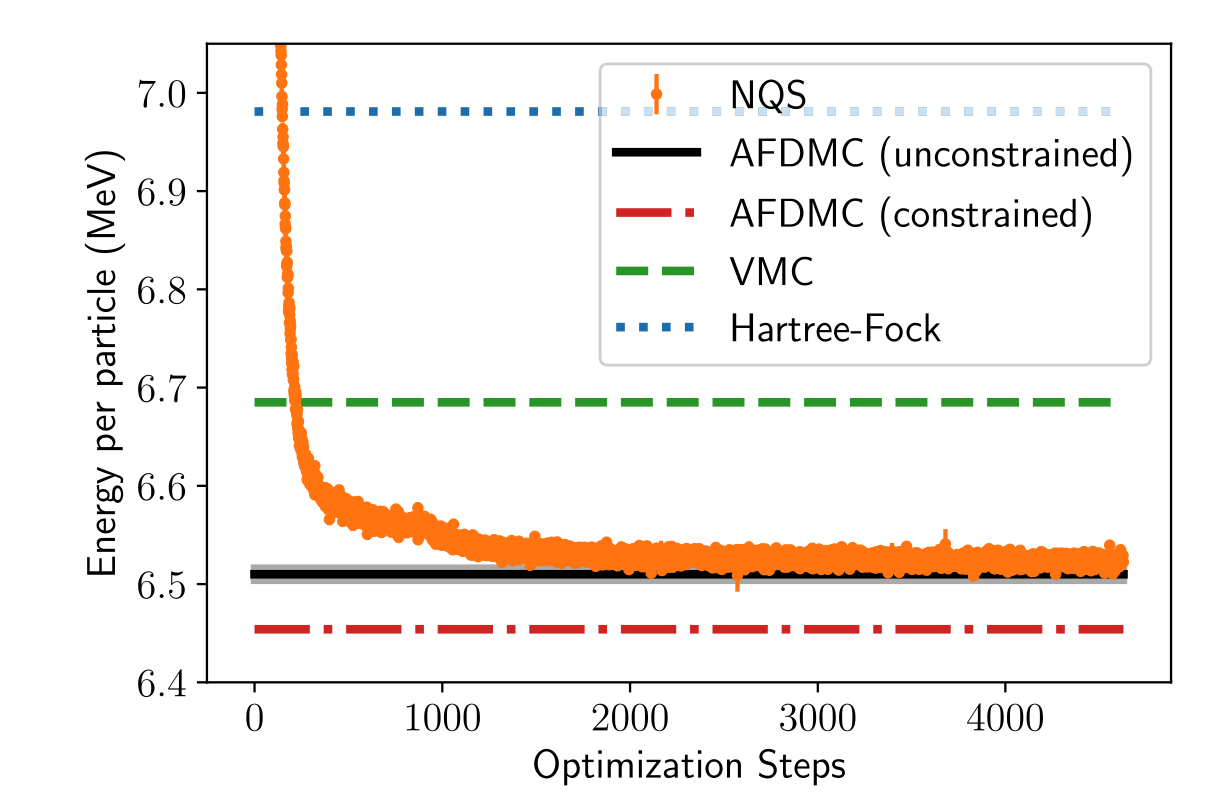
\includegraphics[width=0.9\linewidth]{figures/nmatter.png}}

\vspace{6mm}

\end{block}

% !split
\subsection{The electron gas in three dimensions with $N=14$ electrons (Wigner-Seitz radius $r_s=2$ a.u.), \href{{https://doi.org/10.48550/arXiv.2305.07240}}{Gabriel Pescia, Jane Kim et al.~arXiv.2305.07240,}}

\begin{block}{}

\vspace{6mm}

% inline figure
\centerline{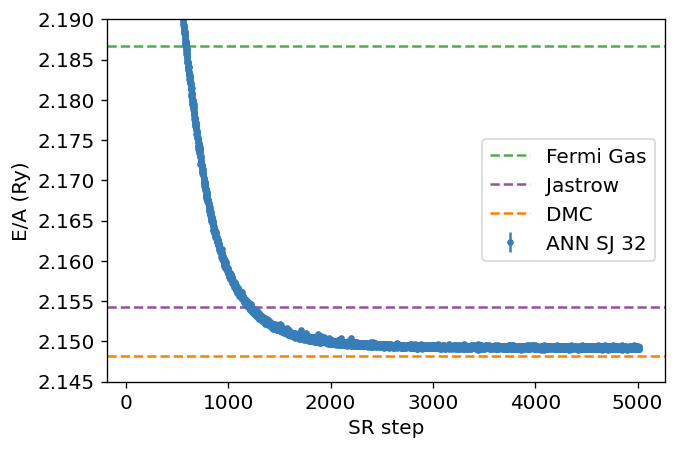
\includegraphics[width=0.9\linewidth]{figures/elgasnew.png}}

\vspace{6mm}

\end{block}

% !split
\subsection{Generative models: Why Boltzmann machines?}

What is known as restricted Boltzmann Machines (RMB) have received a
lot of attention lately.  One of the major reasons is that they can be
stacked layer-wise to build deep neural networks that capture
complicated statistics.

The original RBMs had just one visible layer and a hidden layer, but
recently so-called Gaussian-binary RBMs have gained quite some
popularity in imaging since they are capable of modeling continuous
data that are common to natural images.

Furthermore, they have been used to solve complicated quantum
mechanical many-particle problems or classical statistical physics
problems like the Ising and Potts classes of models.

% !split
\subsection{The structure of the RBM network}

\vspace{6mm}

% inline figure
\centerline{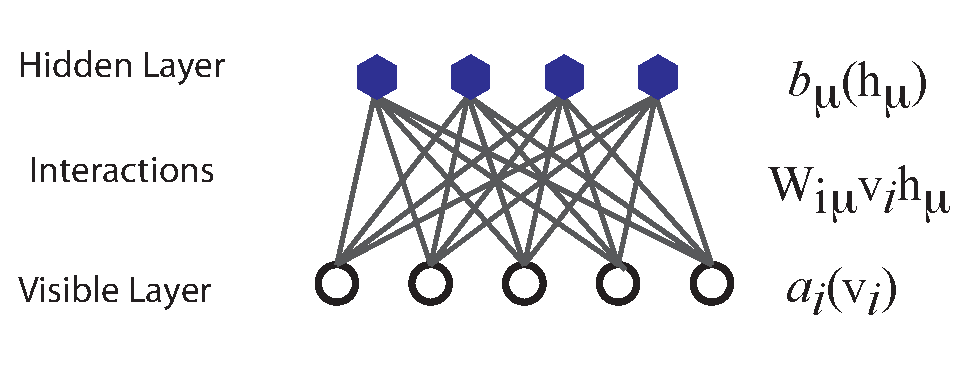
\includegraphics[width=1.0\linewidth]{figures/RBM.pdf}}

\vspace{6mm}

% !split
\subsection{The network}

\textbf{The network layers}:
\begin{enumerate}
 \item A function $\mathbf{x}$ that represents the visible layer, a vector of $M$ elements (nodes). This layer represents both what the RBM might be given as training input, and what we want it to be able to reconstruct. This might for example be the pixels of an image, the spin values of the Ising model, or coefficients representing speech.

 \item The function $\mathbf{h}$ represents the hidden, or latent, layer. A vector of $N$ elements (nodes). Also called "feature detectors".
\end{enumerate}

\noindent
% !split
\subsection{Goals}

The goal of the hidden layer is to increase the model's expressive
power. We encode complex interactions between visible variables by
introducing additional, hidden variables that interact with visible
degrees of freedom in a simple manner, yet still reproduce the complex
correlations between visible degrees in the data once marginalized
over (integrated out).

\textbf{The network parameters, to be optimized/learned}:
\begin{enumerate}
 \item $\mathbf{a}$ represents the visible bias, a vector of same length as $\mathbf{x}$.

 \item $\mathbf{b}$ represents the hidden bias, a vector of same lenght as $\mathbf{h}$.

 \item $W$ represents the interaction weights, a matrix of size $M\times N$.
\end{enumerate}

\noindent
% !split
\subsection{Joint distribution}
The restricted Boltzmann machine is described by a Bolztmann distribution
\[
	P_{rbm}(\mathbf{x},\mathbf{h}) = \frac{1}{Z} e^{-\frac{1}{T_0}E(\mathbf{x},\mathbf{h})},
\]
where $Z$ is the normalization constant or partition function, defined as 
\[
	Z = \int \int e^{-\frac{1}{T_0}E(\mathbf{x},\mathbf{h})} d\mathbf{x} d\mathbf{h}.
\]
It is common to ignore $T_0$ by setting it to one. 

% !split
\subsection{Network Elements, the energy function}

The function $E(\mathbf{x},\mathbf{h})$ gives the \textbf{energy} of a
configuration (pair of vectors) $(\mathbf{x}, \mathbf{h})$. The lower
the energy of a configuration, the higher the probability of it. This
function also depends on the parameters $\mathbf{a}$, $\mathbf{b}$ and
$W$. Thus, when we adjust them during the learning procedure, we are
adjusting the energy function to best fit our problem.

% !split
\subsection{Defining different types of RBMs (Energy based models)}

There are different variants of RBMs, and the differences lie in the types of visible and hidden units we choose as well as in the implementation of the energy function $E(\mathbf{x},\mathbf{h})$. The connection between the nodes in the two layers is given by the weights $w_{ij}$. 

\begin{block}{Binary-Binary RBM: }

RBMs were first developed using binary units in both the visible and hidden layer. The corresponding energy function is defined as follows:
\[
	E(\mathbf{x}, \mathbf{h}) = - \sum_i^M x_i a_i- \sum_j^N b_j h_j - \sum_{i,j}^{M,N} x_i w_{ij} h_j,
\]
where the binary values taken on by the nodes are most commonly 0 and 1.
\end{block}

% !split
\subsection{Gaussian binary}

\begin{block}{Gaussian-Binary RBM: }

Another varient is the RBM where the visible units are Gaussian while the hidden units remain binary:
\[
	E(\mathbf{x}, \mathbf{h}) = \sum_i^M \frac{(x_i - a_i)^2}{2\sigma_i^2} - \sum_j^N b_j h_j - \sum_{i,j}^{M,N} \frac{x_i w_{ij} h_j}{\sigma_i^2}. 
\]
\end{block}

% !split
\subsection{Representing the wave function}

The wavefunction should be a probability amplitude depending on
 $\bm{x}$. The RBM model is given by the joint distribution of
 $\bm{x}$ and $\bm{h}$

\[
        F_{rbm}(\mathbf{x},\mathbf{h}) = \frac{1}{Z} e^{-\frac{1}{T_0}E(\mathbf{x},\mathbf{h})}.
\]

To find the marginal distribution of $\bm{x}$ we set:

\[
        F_{rbm}(\mathbf{x}) =\frac{1}{Z}\sum_\mathbf{h} e^{-E(\mathbf{x}, \mathbf{h})}.
\]

Now this is what we use to represent the wave function, calling it a neural-network quantum state (NQS)
\[
        \Psi (\mathbf{X}) = F_{rbm}(\mathbf{x}),
\]
or we could square the wave function.

% !split
\subsection{Define the cost function}

Now we don't necessarily have training data (unless we generate it by
using some other method). However, what we do have is the variational
principle which allows us to obtain the ground state wave function by
minimizing the expectation value of the energy of a trial wavefunction
(corresponding to the untrained NQS). Similarly to the traditional
variational Monte Carlo method then, it is the local energy we wish to
minimize. The gradient to use for the stochastic gradient descent
procedure is

\[
	C_i = \frac{\partial \langle E_L \rangle}{\partial \theta_i}
	= 2(\langle E_L \frac{1}{\Psi}\frac{\partial \Psi}{\partial \theta_i} \rangle - \langle E_L \rangle \langle \frac{1}{\Psi}\frac{\partial \Psi}{\partial \theta_i} \rangle ),
\]
where the local energy is given by
\[
	E_L = \frac{1}{\Psi} \hat{\mathbf{H}} \Psi.
\]

% !split
\subsection{Extrapolations and model interpretability}

When you hear phrases like \textbf{predictions and estimations} and
\textbf{correlations and causations}, what do you think of?  May be you think
of the difference between classifying new data points and generating
new data points.
Or perhaps you consider that correlations represent some kind of symmetric statements like
if $A$ is correlated with $B$, then $B$ is correlated with
$A$. Causation on the other hand is directional, that is if $A$ causes $B$, $B$ does not
necessarily cause $A$.

% !split
\subsection{Physics based statistical learning and data analysis}

The above concepts are in some sense the difference between \textbf{old-fashioned} machine
learning and statistics and Bayesian learning. In machine learning and prediction based
tasks, we are often interested in developing algorithms that are
capable of learning patterns from given data in an automated fashion,
and then using these learned patterns to make predictions or
assessments of newly given data. In many cases, our primary concern
is the quality of the predictions or assessments, and we are less
concerned about the underlying patterns that were learned in order
to make these predictions.

Physics based statistical learning points however to approaches that give us both predictions and correlations as well as being able to produce error estimates and understand causations.  This leads us to the very interesting field of Bayesian statistics and Bayesian machine learning.

% !split
\subsection{Bayes' Theorem}

Bayes' theorem
\[
p(X\vert Y)= \frac{p(X,Y)}{\sum_{i=0}^{n-1}p(Y\vert X=x_i)p(x_i)}=\frac{p(Y\vert X)p(X)}{\sum_{i=0}^{n-1}p(Y\vert X=x_i)p(x_i)}.
\]

The quantity $p(Y\vert X)$ on the right-hand side of the theorem is
evaluated for the observed data $Y$ and can be viewed as a function of
the parameter space represented by $X$. This function is not
necessarily normalized and is normally called the likelihood function.

The function $p(X)$ on the right hand side is called the prior while the function on the left hand side is the called the posterior probability. The denominator on the right hand side serves as a normalization factor for the posterior distribution.

% !split
\subsection{\href{{https://journals.aps.org/prc/abstract/10.1103/PhysRevC.101.044307}}{Quantified limits of the nuclear landscape}}

Predictions made with eleven global mass model and Bayesian model averaging

\vspace{6mm}

% inline figure
\centerline{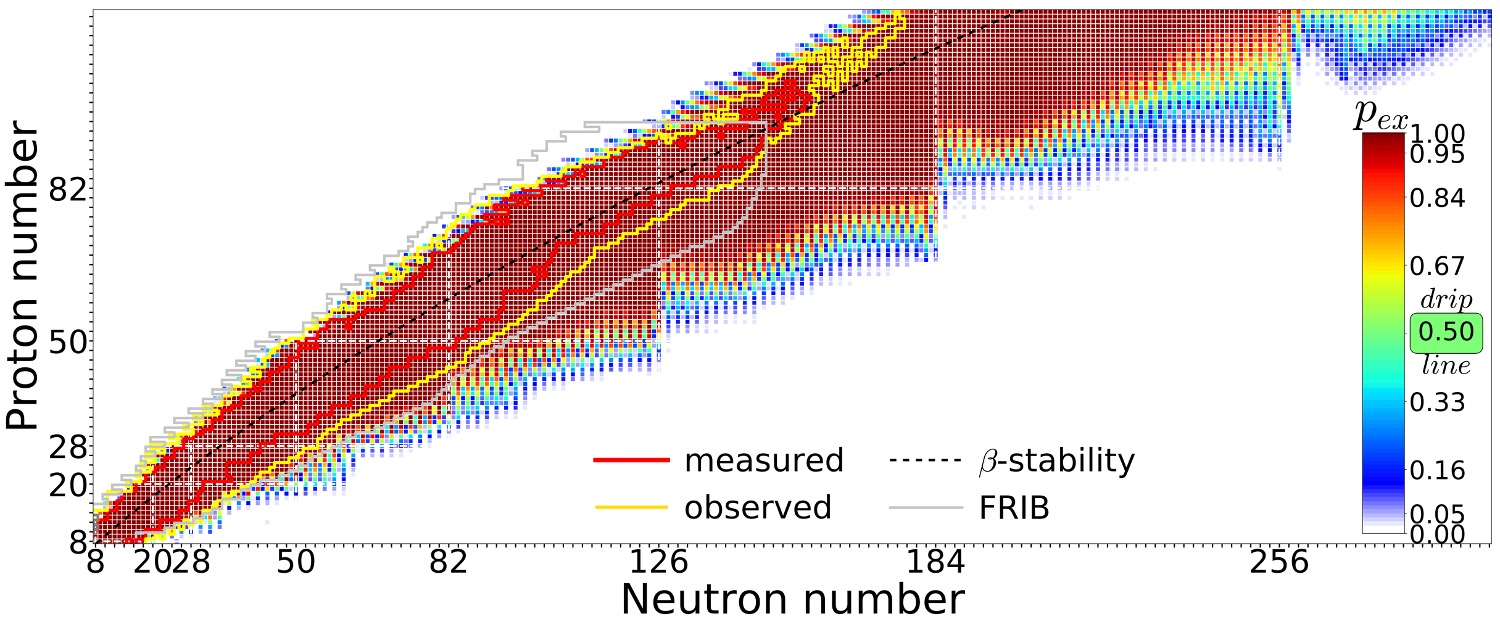
\includegraphics[width=1.0\linewidth]{figures/landscape.jpg}}

\vspace{6mm}

% !split
\subsection{Mathematics of deep learning and neural networks}

Throughout this course we will use the following notations. Vectors,
matrices and higher-order tensors are always boldfaced, with vectors
given by lower case letter letters and matrices and higher-order tensors given by upper case letters.

Unless otherwise stated, the elements $v_i$ of a vector $\bm{v}$ are assumed to be real. That is a vector of length $n$ is defined as
$\bm{x}\in \mathbb{R}^{n}$ and if we have a complex vector we have $\bm{x}\in \mathbb{C}^{n}$.

For a matrix of dimension $n\times n$ we have 
$\bm{A}\in \mathbb{R}^{n\times n}$ and the first matrix element starts with row element (row-wise ordering) zero and column element zero.

% !split
\subsection{Vectors}

We start by defining a vector $\bm{x}$  with $n$ components, with $x_0$ as our first element, as

\[
\bm{x} = \begin{bmatrix} x_0\\ x_1 \\ x_2 \\ \dots \\ \dots \\ x_{n-1} \end{bmatrix}.
\]
and its transpose 
\[
\bm{x}^{T} = \begin{bmatrix} x_0 & x_1 & x_2 & \dots & \dots & x_{n-1} \end{bmatrix},
\]
In case we have a complex vector we define the hermitian conjugate
\[
\bm{x}^{\dagger} = \begin{bmatrix} x_0^* & x_1^* & x_2^* & \dots & \dots & x_{n-1}^* \end{bmatrix},
\]

With a given vector $\bm{x}$, we define the inner product as
\[
\bm{x}^T \bm{x} = \sum_{i=0}^{n-1} x_ix_i=x_0^2+x_1^2+\dots + x_{n-1}^2. 
\]

% !split
\subsection{Outer products}

In addition to inner products between vectors/states, the outer
product plays a central role in many applications. It is
defined as
\[
\bm{x}\bm{y}^T = \begin{bmatrix}
               x_0y_0 & x_0y_1 & x_0y_2 & \dots & \dots & x_0y_{n-2} & x_0y_{n-1} \\
	       x_1y_0 & x_1y_1 & x_1y_2 & \dots & \dots & x_1y_{n-2} & x_1y_{n-1} \\
	       x_2y_0 & x_2y_1 & x_2y_2 & \dots & \dots & x_2y_{n-2} & x_2y_{n-1} \\	       
               \dots &   \dots   & \dots  & \dots & \dots & \dots & \dots \\
               \dots &   \dots   & \dots  & \dots & \dots & \dots & \dots \\	       
	       x_{n-2}y_0 & x_{n-2}y_1 & x_{n-2}y_2 & \dots & \dots & x_{n-2}y_{n-2} & x_{n-2}y_{n-1} \\
	       x_{n-1}y_0 & x_{n-1}y_1 & x_{n-1}y_2 & \dots & \dots & x_{n-1}y_{n-2} & x_{n-1}y_{n-1} \end{bmatrix}	       
\]
The latter defines also our basic matrix layout.

% !split
\subsection{Basic Matrix Features}

A general $n\times n$ matrix is given by 
\[
 \mathbf{A} =
\begin{bmatrix}
               a_{00} & a_{01} & a_{02} & \dots & \dots & a_{0n-2} & a_{0n-1} \\
               a_{10} & a_{11} & a_{12} & \dots & \dots & a_{1n-2} & a_{1n-1} \\
               \dots &   \dots   & \dots  & \dots & \dots & \dots & \dots \\
               \dots &   \dots   & \dots  & \dots & \dots & \dots & \dots \\	       
               a_{n-20} & a_{n-21} & a_{n-22} & \dots & \dots & a_{n-2n-2} & a_{n-2n-1} \\
               a_{n-10} & a_{n-11} & a_{n-12} & \dots & \dots & a_{n-1n-2} & a_{n-1n-1} \end{bmatrix},	       
\]
or in terms of its column vectors $\bm{a}_i$ as
\[
 \mathbf{A} =
\begin{bmatrix}\bm{a}_{0} & \bm{a}_{1} & \bm{a}_{2} & \dots & \dots & \bm{a}_{n-2} & \bm{a}_{n-1}\end{bmatrix}.	       
\]

% !split
\subsection{The inverse of a matrix}
\begin{block}{}
The inverse of a matrix (if it exists) is defined by

\[
\mathbf{A}^{-1} \cdot \mathbf{A} = I,
\]
where $\bm{I}$ is the unit matrix.
\end{block}

% !split
\subsection{Basic Matrix Features}

\begin{block}{Matrix Properties Reminder }


{\footnotesize
\begin{tabular}{ccc}
\hline
\multicolumn{1}{c}{ Relations } & \multicolumn{1}{c}{ Name } & \multicolumn{1}{c}{ matrix elements } \\
\hline
$A = A^{T}$                            & symmetric       & $a_{ij} = a_{ji}$                                                       \\
$A = \left (A^{T} \right )^{-1}$       & real orthogonal & $\sum_k a_{ik} a_{jk} = \sum_k a_{ki} a_{kj} = \delta_{ij}$             \\
$A = A^{ * }$                          & real matrix     & $a_{ij} = a_{ij}^{ * }$                                                 \\
$A = A^{\dagger}$                      & hermitian       & $a_{ij} = a_{ji}^{ * }$                                                 \\
$A = \left (A^{\dagger} \right )^{-1}$ & unitary         & $\sum_k a_{ik} a_{jk}^{ * } = \sum_k a_{ki}^{ * } a_{kj} = \delta_{ij}$ \\
\hline
\end{tabular}
}

\noindent
\end{block}

% !split
\subsection{Some famous Matrices}

\begin{itemize}
  \item Diagonal if $a_{ij}=0$ for $i\ne j$

  \item Upper triangular if $a_{ij}=0$ for $i > j$

  \item Lower triangular if $a_{ij}=0$ for $i < j$

  \item Upper Hessenberg if $a_{ij}=0$ for $i > j+1$

  \item Lower Hessenberg if $a_{ij}=0$ for $i < j+1$

  \item Tridiagonal if $a_{ij}=0$ for $|i -j| > 1$

  \item Lower banded with bandwidth $p$: $a_{ij}=0$ for $i > j+p$

  \item Upper banded with bandwidth $p$: $a_{ij}=0$ for $i < j+p$

  \item Banded, block upper triangular, block lower triangular....
\end{itemize}

\noindent
% !split
\subsection{Matrix Features}

\begin{block}{Some Equivalent Statements }
For an $N\times N$ matrix  $\mathbf{A}$ the following properties are all equivalent

\begin{itemize}
  \item If the inverse of $\mathbf{A}$ exists, $\mathbf{A}$ is nonsingular.

  \item The equation $\mathbf{Ax}=0$ implies $\mathbf{x}=0$.

  \item The rows of $\mathbf{A}$ form a basis of $R^N$.

  \item The columns of $\mathbf{A}$ form a basis of $R^N$.

  \item $\mathbf{A}$ is a product of elementary matrices.

  \item $0$ is not eigenvalue of $\mathbf{A}$.
\end{itemize}

\noindent
\end{block}

% !split
\subsection{Important Mathematical Operations}

The basic matrix operations that we will deal with are addition and subtraction

\begin{equation}
\mathbf{A}= \mathbf{B}\pm\mathbf{C}  \Longrightarrow a_{ij} = b_{ij}\pm c_{ij},
\label{eq:mtxadd}
\end{equation}
scalar-matrix multiplication

\begin{equation}
\mathbf{A}= \gamma\mathbf{B}  \Longrightarrow a_{ij} = \gamma b_{ij},
\end{equation}
vector-matrix multiplication

% !split
\subsection{Matrix-matrix multiplication}
\begin{equation}
\mathbf{y}=\mathbf{Ax}   \Longrightarrow y_{i} = \sum_{j=1}^{n} a_{ij}x_j,
\label{eq:vecmtx}
\end{equation}
and

\begin{equation}
\mathbf{A}=\mathbf{BC}   \Longrightarrow a_{ij} = \sum_{k=1}^{n} b_{ik}c_{kj},
\label{eq:mtxmtx}
\end{equation}
and transposition

\begin{equation}
\mathbf{A}=\mathbf{B}^T   \Longrightarrow a_{ij} = b_{ji}
\end{equation}

% !split
\subsection{Important Mathematical Operations}

Similarly, important vector operations that we will deal with are addition and subtraction

\begin{equation}
\mathbf{x}= \mathbf{y}\pm\mathbf{z}  \Longrightarrow x_{i} = y_{i}\pm z_{i},
\end{equation}
scalar-vector multiplication

\begin{equation}
\mathbf{x}= \gamma\mathbf{y}  \Longrightarrow x_{i} = \gamma y_{i},
\end{equation}
vector-vector multiplication (called Hadamard multiplication)

% !split
\subsection{More on important mathematical operations}
\begin{equation}
\mathbf{x}=\mathbf{yz}   \Longrightarrow x_{i} = y_{i}z_i,
\end{equation}
the inner or so-called dot product  resulting in a constant

\begin{equation}
x=\mathbf{y}^T\mathbf{z}   \Longrightarrow x = \sum_{j=1}^{n} y_{j}z_{j},
\label{eq:innerprod}
\end{equation}
and the outer product, which yields a matrix,

\begin{equation}
\mathbf{A}=  \mathbf{yz}^T \Longrightarrow  a_{ij} = y_{i}z_{j},
\label{eq:outerprod}
\end{equation}

% !split
\subsection{Setting up the basic equations for neural networks}


% ------------------- end of main content ---------------

% #ifdef PREAMBLE
\end{document}
% #endif

